\documentclass[]{article}
\usepackage[T1]{fontenc}

\usepackage{graphicx}
\usepackage[]{hyperref}
\usepackage[french]{babel}

\author{Erwan LEMATTRE, Yannis CHUPIN}
\title{Rapport projet fairness}

\begin{document}

    \tableofcontents
    \newpage

    \section{Introduction}
    Ce projet a pour objectif d'analyser les accidents de la circulation routière afin de pouvoir dire 
    à partir des données d'un véhicule accidenté si l'accident est mortel ou non.
    Les données sont des données libres mises à disposition par le \textit{Ministère de l'intérieur et des 
    Outre-Mer}. Le jeu de donnée correspond aux accidents de 2005 à 2022 en France. Nous allons dans une première 
    partie analyser ces données afin d'extraire les informations utiles à l'apprentissage et de pouvoir repérer 
    d'éventuelles sources de biais pour notre modèle.

    \section{Découverte du jeu de données}
    \subsection{La base de données}
    La base de données est composée de plusieurs tables: \textit{usagers}, \textit{vehicules}, \textit{lieux} et 
    \textit{caracteristiques}. Nous avons joint ces quatres parties pour obtenir un dataframe contenant une 
    cinquantaine de colonnes. 
    Ci-dessous une rapide présentation des différentes données disponibles.

    \begin{center}
        \begin{tabular}{ |c|c| }
            \hline
            \textbf{Attribut} & \textbf{Description} \\
            \hline
            \textit{Num\_Acc} & Numéro d'identifiant de l'accident \\
            \textit{jour mois} & Jour de l'accident, mois de l'accident \\
            \textit{an} & Numéro d'identifiant de l'accident. \\
            \textit{hrmn} & Numéro d'identifiant de l'accident. \\
            \textit{lum} & Numéro d'identifiant de l'accident. \\
            \textit{dep} & Numéro d'identifiant de l'accident. \\
            \textit{com} & Numéro d'identifiant de l'accident. \\
            \textit{agg} & Numéro d'identifiant de l'accident. \\
            \textit{int} & Numéro d'identifiant de l'accident. \\
            \textit{atm} & Numéro d'identifiant de l'accident. \\
            \textit{col} & Numéro d'identifiant de l'accident. \\
            \textit{adr} & Numéro d'identifiant de l'accident. \\
            \textit{lat} & Numéro d'identifiant de l'accident. \\
            \textit{long} & Numéro d'identifiant de l'accident. \\
            \textit{catr} & Numéro d'identifiant de l'accident. \\        
            \hline
        \end{tabular}
    \end{center}

    \subsection{Répartition des données}
    Afin de pouvoir conserver les données utiles pour l'apprentissage nous avons analysé la répartition des 
    différentes données dans notre dataframe.
    Nous avons ainsi pu faire différentes observations. 
    \\
    Voici quelques-unes d'entre elles qui nous sont ensuite
    utiles pour la préparation des données.
    \subsubsection{Catégories de véhicule}
    La base de données nous donne beaucoup de catégories différentes. Nous avons cependant pu remarquer 
    que la majorité des véhicules sont dans seulement 5 catégories.
    \begin{figure}[ht]
        \centering
        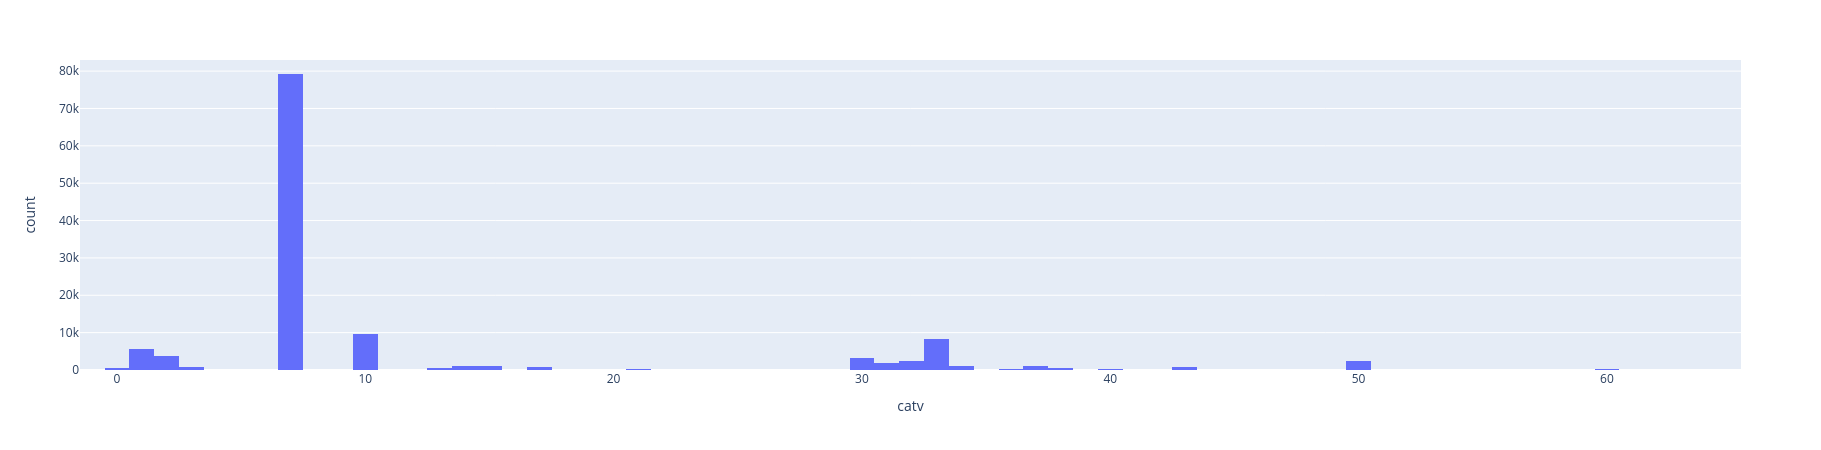
\includegraphics[width=12cm]{./img/catv1.png}
        \caption{Répartition des catégories de véhicules}
    \end{figure}

    \subsubsection{Gravité de l'accident}
    En affichant l'effectif d'accidents mortels nous avons pu remarquer qu'ils ne représentent qu'une 
    infime partie des accidents. Le peu de données sur ces accidents ne nous permet pas l'apprentissage 
    d'un modèle. C'est la raison pour laquelle nous avons décidé de nous intéresser non pas à la mortalité 
    à l'échelle d'une personne mais plutôt à l'échelle d'un accident. Nous nous mettons pour cela au niveau d'un 
    véhiule car cela nous permet de conserver plus d'informations (à l'échelle d'un accident on aurait 
    dû enlever trop d'informations pour conserver seulement les attributs plus généraux à l'accident).

    \begin{figure}[ht]
        \centering
        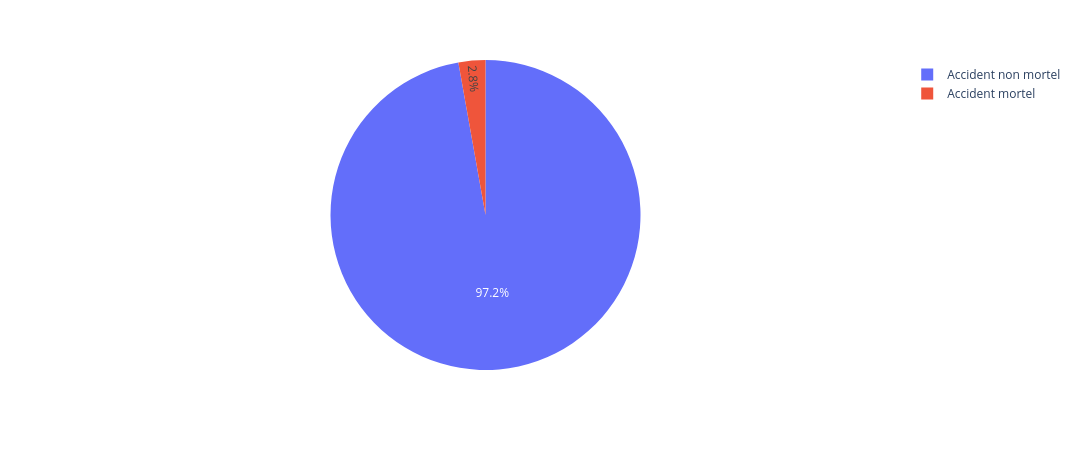
\includegraphics[width=12cm]{./img/grav1.png}
        \caption{Proportion d'accidents mortels}
    \end{figure}

    \section{Préparation des données}
    \subsection{Préparation des attributs utiles}
    À partir des observations précédentes, nous avons supprimé les attributs moins intéressant pour l'apprentissage 
    et nous avons modifié certains attributs afin d'en extraire les informations intéressantes.
    \\
    Les attributs supprimés sont: \textit{voie}, \textit{v1}, \textit{v2}, \textit{pr}, \textit{pr1}, \textit{lartpc},
     \textit{larrout}, \textit{num\_veh}, \textit{occutc}, \textit{adr}, \textit{senc}, \textit{etatp}, \textit{actp}, 
     \textit{manv}, \textit{jour}, \textit{com}, \textit{hrmn}, \textit{motor}, \textit{place}, \textit{vosp}, \textit{locp}.
    \\\\
    Nous avons effectué les modifications suivantes:
    \begin{itemize}
        \item Création d'un attribut \textit{mortal} qui vaut 1 si le véhicule est impliqué dans un accident mortel, 0 sinon.
        \item À partir de l'attribut \textit{sexe} nous avons créé un attribut \textit{sexe\_conducteur} qui garde seulement 
                le sexe du conducteur du véhicule.
        \item Nous avons utilisé l'année de naissance et l'année de l'accident pour récupérer l'âge du conducteur.
        \item L'attribut \textit{vma} a été découpé en 4 catégories de vitesse.
        \item Pour les attributs \textit{catv} et \textit{vatr} nous avons gardé les valeurs le plus représentées dans la base de données.
    \end{itemize}

    \subsection{One Hot Encoding}
    Une grande partie des attributs sont des attributs numériques mais sont tout de même des attributs catégoriels.


    \section{Analyse des données}
    

    \section{Apprentissage}

    \section{Audit du modèle}



\end{document}